\ofsubsection{Encicolpédia de Ivalice}
%
\ofquote{"Nomes não importam. O que importa é como você vive sua vida."}{Ramza Belouve}\\\\
%
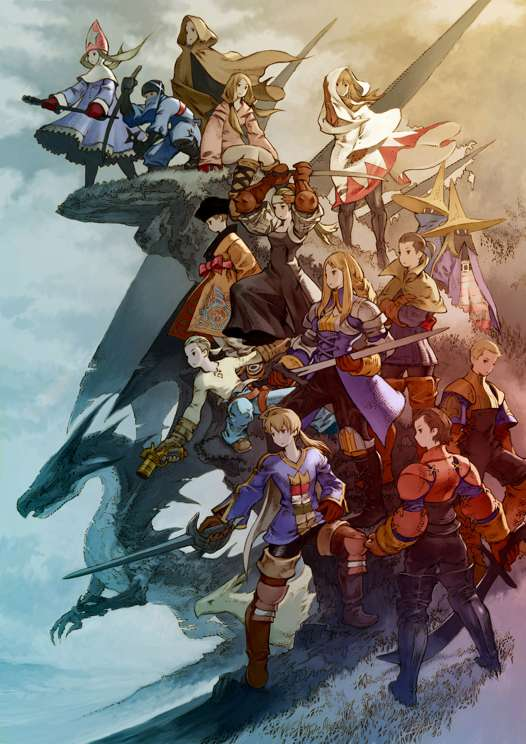
\includegraphics[width=\columnwidth]{./art/worldbook/everyone.jpg}
%
\ofrow
%
A \accf{Encicolpédia de Ivalice} é um documento que compreende o cenário do jogo eletrônico Final Fantasy Tactics. 
Ela inclui muitos detalhes sobre sua história e geografia a fim de lhe ajudar a criar suas próprias aventuras nesse mundo.
Este suplemento é uma versão atualizada da original, escrita por Bruno Carvalho, Paul (Papa Quackers) e Hywel Williams em 2017, incluindo regras para o sistema de jogo de interpretação de Final Fantasy 4º edição~(\accf{FFRPG~4e}).
O conteúdo e ideias apresentadas nesta versão da enciclopédia, é um sistema agnóstico e, assim sendo, aplicável a outros RPGs de mesa.
%
\ofpar
%
\accf{Final Fantasy Tactics}~(FFT) é um título secundário da série principal de Final Fantasy. 
Diferente da maioria de títulos secundários, esse conseguiu ser um grande jogo, tendo recebido aclamação universal após seu lançamento e a opinião crítica sobre ele só tem melhorado ao longo do tempo.
Este é o primeiro jogo da série de Final fantasy tactics, lançado no Japão em Junho de 1997 e nos Estados Unidos, em Janeiro de 1998.
O jogo combina elementos da temática da série de jogos eletrônicos de Final fantasy, com um motor de jogabilidade e sistema de batalha diferente daqueles anteriormente vistos na franquia.
Em contraste aos outros títulos da série da era 32-bits, esse título usa um campo 3D jogável, rotativo e isométrico, com sprites de personagens em bitmap.
Para muitos jogadores de Final fantasy, este representou sua primeira incursão nos jogos de RPG estratégicos, com suas próprias características e convenções, já estabelecidas por vários outros jogos que vieram antes, como Shining force, a série Langrisser e Tactics ogre.
Por isso e para celebrar o aniversário de 20 anos do lançamento original no Japão deste clássico cult, esta enciclopédia nasceu.
%
\vfill
%
O Final Fantasy Tactics usa um grid de batalha isométrico e tri-dimensional.
Essa diferença em funcionalidade gerou um tipo de jogo que estava mais aparentado ao xadrez, do que com o combate linear para frente e para trás, tradicional dos outros jogos da franquia.
Ao invés de ter seis personagens que eram centrais para a trama, que se juntavam ao seu grupo após um período, você tinha um único personagem principal que ocasionalmente se juntaria, pela história, a outros personagens importantes, que partiriam e se juntariam novamente às exigências da trama.
Normalmente, grande parte de seu grupo de aventura era composto por personagens intercambiáveis e sem roteiro, cuja aparência mudaria completamente a depender de qual \accf{profissão} lhes fosse selecionada.
A progressão delas neste sistema é bem parecida àquela dos jogos de Final Fantasy antigos, na qual havia várias profissões para se escolher, mas fundamentalmente diferente em como cada uma delas seria desbloqueada.
Ao invés de obter cristais que garantiriam certas profissões automaticamente, a você era dada duas profissões iniciais e expandiria às demais a partir delas.
O progresso de sua profissão revela outras e se você ganhar vários níveis em várias delas, a experiência acumulada pode revelar uma outra.
Este sistema envolve muita alternância de profissões e, é claro, uma pequena quantidade de mapeamento de classe para determinar qual profissão desbloqueia qual.
%
\vfill
%
\ofquote{"Os melhores caminhos, nem sempre levam aos melhores resultados."\\}{Delita Hyral}\\\\
%
A estória de Final Fantasy Tactics se desenrola após \accf{A guerra dos 50 anos}.
O reino de \accf{Ivalice} é abundante em discrepâncias políticas e econômicas entre as classes alta e baixa.
Este problema é composto pela recente morte do rei, cujo único herdeiro é uma criança e a necessidade de um regente para governar em seu lugar.
As pessoas estão entre o príncipe Goltana e o príncipe Large, conhecidos como o Leão Negro e o Leão Branco, respectivamente.
Isto leva à trama principal do jogo, conhecida como \accf{A guerra do Leão}, na qual você toma o papel de \accf{Ramza Beoulve}.\\
Como implica o nome, A guerra do Leão foram conflitos entre os dois príncipes na tentativa de se tornarem o regente.
Ramza é um jovem nobre que participa de muitos momentos da guerra, descobre as maquinações e corrupção escondidas dentro da mais poderosa igreja e acabar por entender a súplica das pessoas comuns.
Ele foi um fator decisivo na resolução da guerra, embora ativamente apagado da história.
%
%
%
\clearpage
%
\ofsubsubsection{História}
%
\accf{O início (10.000 B.C. -- 2.000 B.C.)}\\
Durante este período, estimado de 10.000 a 2.000 B.C. no calendário Ajoriano, a maioria da humanidade vivia na costa sudoeste do que viria a ser conhecida posteriormente como Kaladis.
A maioria das pessoas deste tempo eram tribos simples de caçadores-coletores. À medida em que chegava ao seu fim, no entanto, a metalurgia foi desenvolvida assim como o estudo básico sobre magia.
Infelizmente, há pouquíssimos registros deste período. Parcialmente graças à falta de linguagem escrita, a qual foi primeiro desenvolvida durante o império Ronan, embora haja raras ruínas deixadas para trás, que têm sido encontradas em diversas partes de Kaladis.
Durante este período, os países que mais tarde se tornariam Kaladis e Mizuno, foram primeiros estabelecidos. Ivalice, Romanda e Ordalia foram primeiro estabelecidas durante o império Ronan.
%
\ofpar
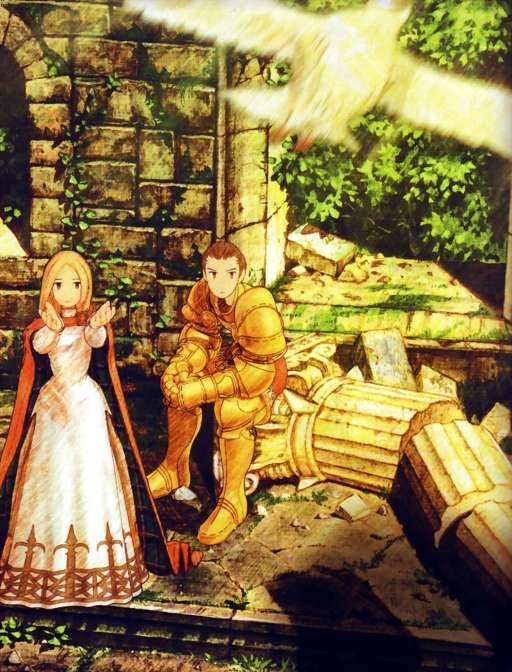
\includegraphics[width=\columnwidth]{./art/worldbook/ovelia.jpg}
\ofpar
%
\accf{O império Ronan (2.000 B.C. -- 700 B.C.)}\\
A história data a primeira civilização de fato como sendo o império Ronan; este que cresceu de uma humilde vila campestre, próxima a Zeltana, até um enorme império que cobria a maior parte do que se tornaria Ivalice e partes de Romanda e Ordalia, próximo ao seu fim, que foi estimado entre 700 e 600 B.C..
Não muito é conhecido sobre esse império misterioso, salvo que dominaram o uso da magia, mesmo se comparado ao nível usado pelos mais poderosos magos atuais.
Ainda mais misteriosa é a causa de sua derrocada.
O palácio de Ronan, o centro do império, esteve de pé até sua descoberta durante A guerra do Leão, um mito em si.
Várias ruínas importantes originadas desta era, incluem a caverna de Matoya, a torre de babel, a torre miragem e, é claro, o \accf{Palácio de Ronan}.
O império de Ronan foi o primeiro país a desenvolver a linguagem escrita, com Mizuno, seguindo com sua própria logo em seguida, a conhecida Nihonjin.
%
\ofpar
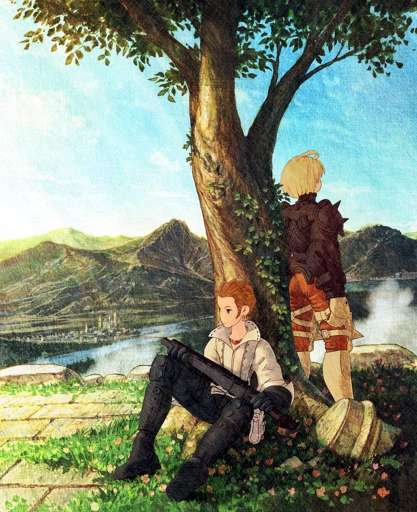
\includegraphics[width=\columnwidth]{./art/worldbook/tree.jpg}
\ofrow
%
\accf{A era do mito (700 B.C. -- 50 B.C.)}\\
Em seguida à derrocada do império de Ronan, os territórios estilhaçados em quatro países separados: Melmond, o reino de Barron, o reino de Kushuka e o império Palamecian.
Assim como seu antecessor, essas quatro nações cobriram toda Ivalice e começaram a fazer estradas até as áreas que viram a se tornar Romanda e Ordalia posteriormente.
Este período é amplamente conhecido como a era do mito, em parte devido à quantidade de ruínas fantásticas deixadas para trás, assim como, o nível de tecnologia desenvolvido.
\accf{Reino de Barron}  era um reino cujo poderio militar rivalizava muitas das outras nações durante a era do mito.
Barron mantinha uma grande quantidade de cavaleiros de elite, assim como, as tanto conhecidas armada de aeronaves.
Barron cobria muito do que se tornaria Gallione, Fovoham e Lesalia ocidental.
Comparado aos seus vizinhos, o \accf{Reino de Kukusha} era o centro de comércio e mercadores de todas as partes ali iam para vender suas mercadorias.
Infelizmente, para o próprio país, sua nobreza governava com mão de ferro e pouca preocupação para com as pessoas.
Após anos de abuso dos cofres da nação, a família real foi destronada por uma enorme revolução.
No mapa moderno, Kukusha ocuparia muito da Lesalia central e a maioria de Zeltania.
Assim como seus vizinhos, o \accf{Império Palamecian} tinha uma especialidade, chamada de tecnologia.
Ele foi o primeiro a desenvolver as aeronaves e manter uma frota que era equivalente à armada de Barron.
Além das aeronaves, Palamecia também foi o primeiro a desenvolver armas de fogo e usar munições mágicas, assim como seus "Golens de guerra", poderosos robôs usados como primeira linha de soldados e guardas.
O império cobria o que se tornaria Lionel.
Muitos historiadores acreditam que sua capital está bem abaixo da Cidade mecânica de Goug. 
palamecia também foi o primeiro a desenvolver dispositivos movidos a vapor, além dos primeiros a desenvolver a ciência das magitec, que envolve a fusão entre magia e máquina.
\accf{Melmond} era uma nação isolada no longínquo oriente, a qual mais tarde se tornaria Ordalia.
Mais do que os outros países, Melmond abraçou o estudo da magia totalmente, apoiando academias dedicadas a ensinar as artes arcanas à alunos interessados.
Outros estudos como história, filosofia e literatura também eram bastante populares entre seus cidadãos.
Infelizmente, Melmond era considerada por muitos de seus vizinhos como sendo parceiros das forças de Lucavi, devido ao seu poderia mágico.
Assim como o império Ronan antes deles, todos os quatro reinos da era do mito foram destruídos sob circunstancias desconhecidas.
A \accf{Brava estória do Zodíaco} primeiro surgiu durante esta era.
Para aqueles que não a conhecem, a Brava estória do Zodíaco é uma lenda sobre um rei maligno que obteve os poderes de Lucavi, a cerca do ano de 500~B.C..
Mas Lucavi matou o rei e causou grande destruição pelo mundo.
No fim, um pequeno grupo de 12 heróis se juntaram e usaram as sagradas pedras do zodíaco para se tornarem os Bravos Zodíacos.
Eles conseguiram derrotar Lucavi e supostamente restauraram a ordem. Após a derrota do inimigo, o \accf{Sacro império de Ydoran} foi fundado, emergido das ruínas do velho reino de Barron.
O império participou de diversas guerras, eventualmente derrotando e conquistando tanto Palamecia quanto Melmond.
%
\vfill
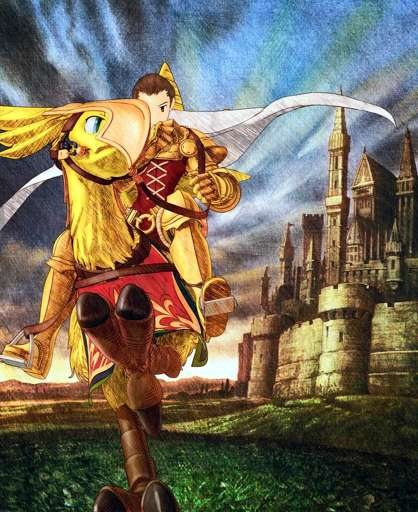
\includegraphics[width=\columnwidth]{./art/worldbook/delita2.jpg} 	
%
\newpage
%
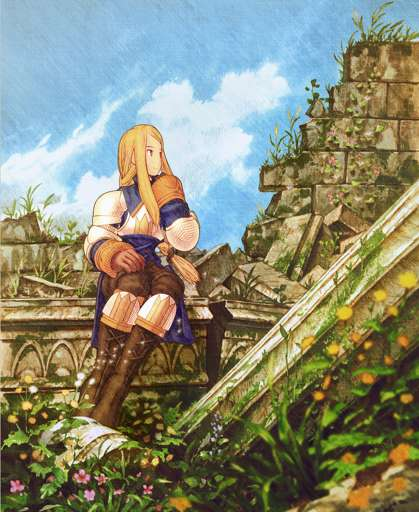
\includegraphics[width=\columnwidth]{./art/worldbook/agrias.jpg}
\ofpar
%
\accf{Vida e morte de Santo~Ajora (50 B.C. -- 1 B.C.)}\\
O calendário Ajoriano começa seu primeiro ano com a morte do \accf{Santo Ajora} e o início do \accf{Cataclismo}.
No momento em que Ajora Glabados surgiu, três dos quatro impérios da era do mito já haviam sido conquistados pelo Sacro império de Ydoran, e o império de Kukusha era somente outro estado resistindo ao poder de seus vizinhos.
As terras que uma vez foram Melmond, jaziam abandonadas e desoladas, onde os refugiados das guerras santas, que viriam a seguir o surgimento da igreja de Glabados, somente se estabeleceriam novamente, vários séculos depois.
Quando Ajora Glabados era jovem, um dia ele apareceu, andou até um poço e profetizou que "logo, a calamidade cairá sobre esta terra. Estou agora, selando este poço e ninguém poderá beber dele." Vários dias depois, a "Morte negra" assolou Zeltenia.
As pessoas que beberam do poço contaminado ficaram doentes e morreram uma após a outra.
Entretanto, somente as famílias que acreditaram nas palavras do Santo Ajora sobreviveram e não sucumbiram à doença.
Desde então, Santo Ajora foi venerado como a "Criança milagrosa" ou "O filho de Deus".
Logo após estes eventos, a palavra de um novo messias se espalhava, aquele que guiaria Ivalica para fora do caos nascido dos anos de guerra.
Ao Santo Ajora chegar aos 18 anos, ele já tinha ganhado uma comunidade de seguidores devotados.
Assim como nos anos passados, outro rei ambicioso tentou invocar Lucavi.
O imperador havia criado um exército imenso na esperança de garantir toda Ivalice sob o controle do Sacro império de Ydoran.
Mais uma vez, um novo grupo de Bravos Zodíacos foi criado e unido pelo Sto. Ajora a fim de derrotar o novo Lucavi.
A despeito de sua crescente fama, Ajora havia feito muitos inimigos.
O Sacro império de Ydoran temia sua ascensão ao poder; Temiam sua pregação da vinda de Deus.
O fé do \accf{Clero de Pharism} era a religião predominante e mesmo tendo grande influência, temiam o poder de Ajora. A conclusão é óbvia.
Santo Ajora foi capturado com uma dica secreta de Germonik, seu 13º apóstolo.
Ele foi executado no campo de execução de Golgollada.
No entanto, como era o "Filho de Deus".
A ira divina caiu sobre Pheisias e o Cataclismo se iniciou, uma série de fenômenos vulcânicos e sísmicos que chocaram o mundo pelos próximos 25 anos.
O Cataclismo era em geral, assumido como sendo a causa por trás da perda da maioria das tecnologias avançadas de Ivalice, embora o jogo nunca tenha afirmado isso.
Também destruiu as últimas duas raças, os "alados" (possivelmente os aegyl), os moogles (como dito no Matagal de Siedge) e na Cidade mecânica de Goug e, caso o mito de ivalice seja verdade, ameaçou a humanidade, levando alguns a acreditarem que isso foi o responsável pelo desaparecimento das raças não humanas de Ivalice.
O afundamento de Mullonde, envolvendo o afogamento de um estado inteiro da península Ivaliciana, também se relaciona a isso.
O Cataclismo criou um continente flutuante, destruiu Eureka e a fortaleza dos julgamentos.
Segundo a lenda, o herói rei, Mesa, salvou a humanidade de seus efeitos.
%
\ofpar
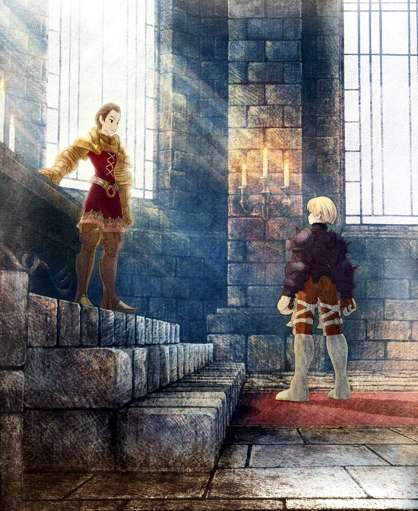
\includegraphics[width=\columnwidth]{./art/worldbook/delita.jpg}
\ofpar
%
\accf{A Ascêncão da igreja de Glabados (25 A.C -- 1112 A.C.)}\\
Em seguida à morte do Sto. Ajora, seus apóstolos restantes estabeleceram uma nova igreja em seu nome e homônima a este: a \accf{Igreja de Glabados}.
Logo após seu estabelecimento, ela foi capaz de cooperar com nações em guerra, que surgiram após o Cataclismo e o subsequente colapso do Sacro império de Ydoran, em um tratado de paz que estabeleceu a família \accf{Atkasha} como os governantes de Ivalice.
Como parte do acordo, Limberry foi anexada a Ivalice.
Apesar do fim da guerra de canetas entre as nações remanescentes, uma nova guerra fria se desenvolveu entre os seguidores restantes do clero de Phara e a recém formada igreja de Glabados.
Como o Pharism foi enfraquecido graças à tragédia que levou à destruição do império de Ydoran, a igreja de Glabados não teve dificuldades ao expulsar o clero de Phara e seus seguidores de Ivalice. Eles iriam, ao longo dos próximos 300 anos, ajudar a criar a nação de Ordalia, ao leste.
A igreja de Glabados, durante seus primeiros 1.000 anos de existência, foi muito poderosa. Graças à sua mão de ferro, ajudou a criar várias facções dissidentes diferentes de sua religião, incluindo a igreja de Argades, a qual se tornaria a religião oficial do império de Romanda.
%
\ofpar
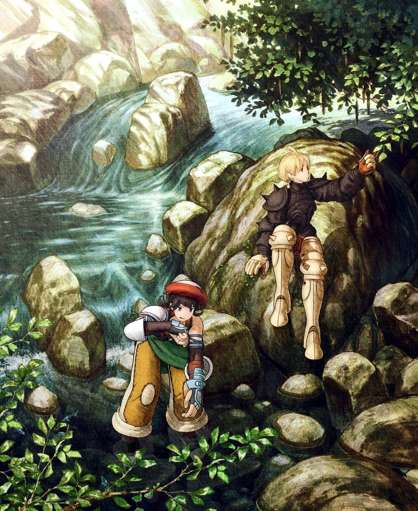
\includegraphics[width=\columnwidth]{./art/worldbook/luso.jpg}
\ofpar
%
\accf{A guerra dos cinquenta anos (1113 A.C -- 1163 A.C.)}\\
Em 1113, o rei Denamda II governou Ivalice, enquanto o rei Devanne III, o reino vizinho, Ordalia.
Três ordens de cavaleiros defendiam Ivalice: a Ordem de cavaleiros do céu nortenho, liderado pelo pai de Ramza, \accf{Barbaneth Beoulve}, a Ordem de cavaleiros do céu austral, liderados por \accf{Cidolfus orlandeau} e a Ordem de cavaleiros do céu oriental, liderados por \accf{Goffard Gaffgarion}.
Gustav Margiff e \accf{Weigraf Folles} serviram à Ordem do céu nortenho.
Conflitos surgiram em Zelmonia, uma província uma vez independente, próxima à borda de Ivalice e agora sob o comando Ordaliano.
A cerca de um século atrás, Ordalia invadiu e anexou Zelmonia.
Ivalice secretamente provia meios para enfraquecer Ordalia; Entretanto, os nobres de Zelmonia decidiram em segredo, peticionar pela intervenção direta do rei Denamda.
O rei Devanne III morreu sem nomear um sucessor.
Seu primo Varoi VI foi então nomeado, mas o rei Denamda II proclamou a si mesmo como o herdeiro de direito, sendo tio de Devanne, e declarou guerra contra Ordalia.
O rei Denamda II liderou o exército de Ivalice em direção à capital de Ordalia, Viuria.
No caminho, os cavaleiros das três Ordens lutaram valentemente, vencendo batalha após batalha.
À medida que se aproximavam da fronteira de Ordalia, o rei Denamda II adoeceu e morreu logo em seguida, nunca sendo capaz de retornar ao seu reino. O exército Ivaliciano ficou confuso e perdido devido à morte de seu líder e Ordalia aproveitou a oportunidade para fortalecer o seu próprio e defender suas fronteiras. 
%
\vspace*{0.5cm}
%
\begin{center}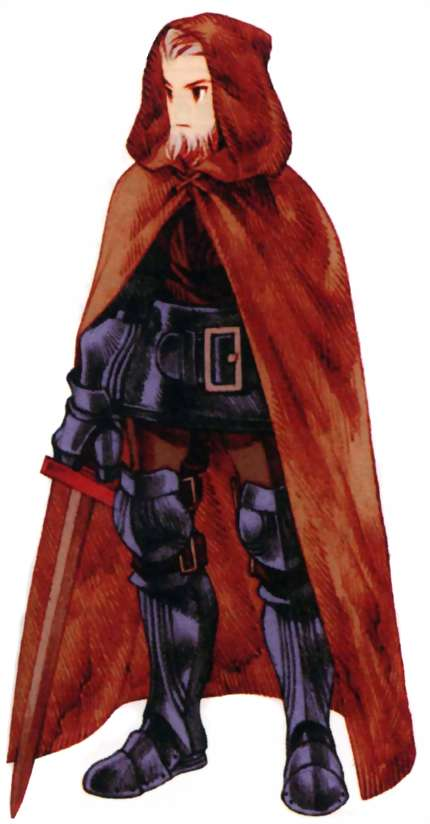
\includegraphics[width=0.65\columnwidth]{./art/worldbook/cid.jpg}\end{center}
%
\vspace*{0.5cm}
%
A guerra foi feroz, alcançando um impasse.
Um sucessor ao Denamda II, o Denamda III, foi rapidamente entronado para substituir seu pai.
Durante o impasse, os exércitos d eRoamnda cruzaram o estreito de Rhana numa invasão à Ivalice.
Romanda era uma nação militar, liderada por um parente de sangue do rei Varoi VI. 
O rei Denamda IV e seu exército Ivaliciano seguraram a invasão com o auxílio do governante de Fovea, o grande Duque Gerrith Barrington e seu esquadrão de assassinato, o Khamja.
Após três anos de luta, Romanda recuou.
O rei Denamda IV foi um guerreiro destemido, que liderou seus exércitos em batalha pessoalmente, contra as forças de Romanda e Ordalia combinadas.
O surto da Morte Negra dentro de Roamnda também levou a sua retirada. Assim sendo, Ivalice continuou em guerra contra Ordalia.
Denamda IV morreu subitamente, acredita-se que assassinado e foi sucedido pelo rei Ondoria Atkasha III, embora o rei foi um homem de mente fraca e inapto para governar, por isso todas as suas decisões eram feitas pela \accf{rainha Louveria}.
O governante de Ordalia, Varoi VI, também faleceu e foi substituído pelo príncipe Lennard.
Devido à fraqueza de Ondoria, Ordalia forçou Ivalice a cessar a luta.
A última batalha entre os reinos aconteceu em Zeltenia, e embora os cavaleiros das ordens tenham lutado bravamente, Ordalia venceu e ocupou a província.
Ivalice e Ordalia concordaram em uma paz mútua, embora diga-se à boca pequena que na realidade Ivalice se rendeu.
Após a guerra dos cinquenta anos, Ivalice sofreu uma grande perda na medida em que pessoas nutriam péssimos sentimentos e dessatisfação quanto aos nobres e a família real, que os colocaram numa guerra sem sentido.
Fazendeiros realizaram motins e se revoltaram, além de muitos viraram a casaca para se juntar à \accf{Brigada cadáver}.
A economia de Ivalice sofreu, como os pagamentos não poderiam ser dados aos cavaleiros que lutaram na guerra devido aos gastos com armas e defesas.
Muitos deles foram dispensados do exército e com menos comida e dinheiro, havia alto desemprego e deslealdade para que as facções governantes crescessem.
Os dois filhos do rei Ondoria morreram, fazendo com que ele adotasse sua irmã mais nova, a \accf{princesa Ovelia}, como sua filha.
Logo após, a raina Louveria deu à luz o príncipe Orinus, causando um conflito sobre quem deveria ser o sucessor do rei, preparando o campo para a Guerra dos Leões.
Os rumores da fraca saúde do rei Ondoria se espalham.
Desde seu colapso, durante a celebração de nascimento do príncipe Orinus, ficou óbvio que ele estava perto da morte.
Seus conselheiros, o conselho de mordomos, deram notícias que o rei estava melhorando, mas o povo conhecia a verdade. Logo os rumores vazaram de que a rainha Louveria e outros nobres discutiram sobre sua sucessão.
Goffard Gaffgarion foi dispensado do Céu oriental, e Gustav do Céu nortenho, ambos acusados de má conduta durante a guerra.
Gaffgarion se voltou à vida de mercenário, clamando lealdade à quem pagar mais.
%
\vfill
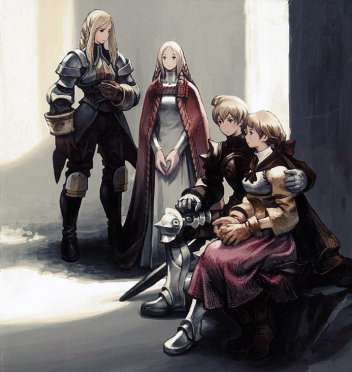
\includegraphics[width=\columnwidth]{./art/worldbook/belouve.jpg}
%
\clearpage
%
\accf{A Guerra dos Leões (1164 A.C -- 1166 A.C.)}\\
A Guerra dos Leões foi lutada entre a Ordem dos cavaleiros do céu nortenho, do \accf{Duque Larg}, sob a bandeira do leão branco e a Ordem de cavaleiros do céu austral, do \accf{Duque Goltanna}, sob a bandeira do leão negro.
O rei Ondoria Atkasha III morreu devido à Morte Negra quando o seu herdeiro, o príncipe Orinus, tinha apenas 2 anos.
Um regente foi solicitado para governar no lugar do príncipe e ambos os duques, generais condecorados da Guerra dos cinquenta anos, foram nomeados como regentes.
Uma das principais razões por trás da guerra foi a de que, o cisão entra a rainha Louveria e os nobres de Ivalice.
Ela era considerada como uma rainha maluca pelo poder, que desejava seu descendente no trono para que assim ela pudesse governar o reino.
O Conselho dos nobres, a fim de evitar que ela reivindicasse influencia pelo reino, apontou o duque Goltana como seu candidato preferido à regência.
%
\ofpar
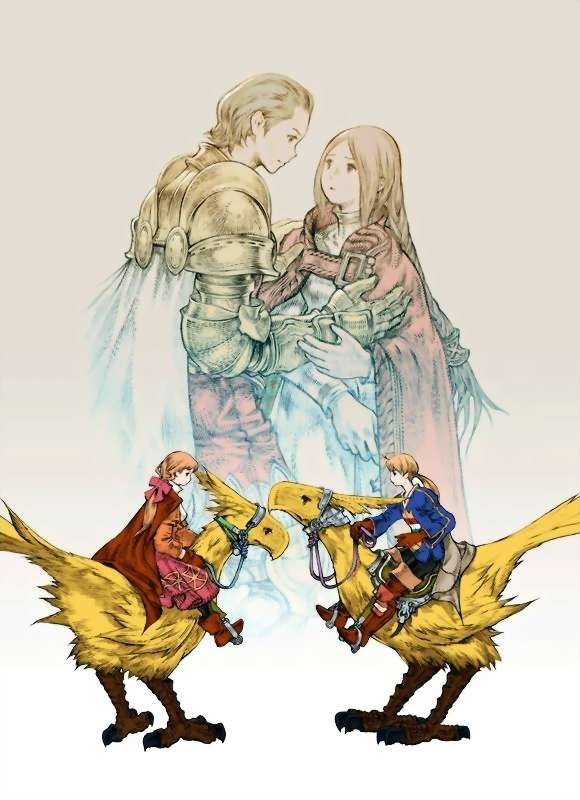
\includegraphics[width=\columnwidth]{./art/worldbook/cover.jpg}
\ofpar
%
A primeira grande batalha da Guerra dos leões, a batalha das planícies de Lesalia, foi um ataque massivo de cavaleiros de Chocobo, de Gallione nas planícies do sul da Cidade real de Lesalia, onde o palácio real foi construído.
O céu austral foi expulsa da cidade e forçada a suas fortalezas de Forte Besselat e o Castelo Limberry.
A vitória levou ao planos da Ordem austral a na maioria girar em torno de um ataque à Lesalia, ao enviar um exército liderado por Cidolfus Orlandeau para tomar a cidade, mas foram expulsos.
Outra tentativa da Ordem austral atacar Lesalia culminou na batalha de Groffovia, lutada nas planícies entre Limberry, que era em geral pró Ordem austral, e Lesalia propriamente dita.
A batalha foi inconclusiva, mas dentro de três meses, as causalidades alcançaram 40.000, minando o pouco suporte popular que a guerra já tinha.
Por volta desse tempo, a rainha Louveria e o chanceler Glevanne foram acusados de sequestrar a princesa Ovelia, a fim de permitir que o duque Larg ascendesse ao trono.
Além disso, a fome assolou Zeltennia, Limberry, Galionne e Fovoham devido à seca, causando mortes por inanição em massa entre os civis.
As perdas mantidas pelo Céu austral pioraram pela batlaha das planícies de Fusse, na qual o marquês Elmdore foi morto por uma flecha perdida.
Ele foi possuído pelo Lucavi \accf{Zalera} e lutou pelos cavaleiros templários na batalha do castelo Riovanes.
Apesar da morte de soldades incontáveis, a guerra chegou a um impasse.
%
\ofpar
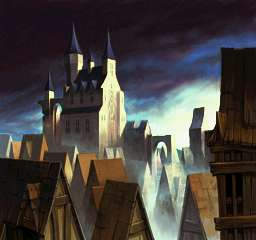
\includegraphics[width=\columnwidth]{./art/worldbook/riovanes.jpg}
\ofpar
% 
O Céu nortenho planejou partir para um ataque de tudo ou nada ao Forte Besselat, planejando tomar e usá-lo como base do qual eles poderiam fomentar guerra total contra os suprimentos de comida da Ordem austral.
A batalha decisiva da guerra foi a batalha do Forte Besselat, na qual Ramza Beoulve interveio abrindo as comportas da barragem, levando a batalha a um cessar indecisivo. 
Barich Fendsor, um dos cavaleiros templários, liberaram veneno de fungo de musgo no ar, enfraquecendo severamente ambos os lados.
Na confusã, ambos os duques foram assassinados por seus respectivos traidores, Larg por \accf{Dycedarg Beoulve} e Goltanna por \accf{Delita Heiral}.
Como originalmente planejado, a igreja ofereceu mediadores.
Apesar da perda de ambos os líderes das Ordens, seus exércitos ainda eram fortes e reticentes à ideia.
Isto pode ter sido a causa da intervenção de Ramza, ao passo que sem isso, ambos os lados teria sofrido grandes perdas se a comporta não tivesse sido aberta.
Ramza Beoulve viajou com seus companheiros ao monastério Orbonne a fim de parar os cavaleiros templários e a trama de Lucavi pela \accf{ressurreição de Ulmtima}.
Derrotando as forças da igreja que ousaram os parar, eles foram teleportados para o cemitério de aeronaves abaixo da necrópole de Mullonde e destruíram Ultima, o alto serafim, que desejava destruir Ivalice.
O destino deles após esse feito é um mistério.
A guerra finalmente terminara com os dois lados combalidos.
Com os dois duques mortos, a rainha Louveria aprisionada no Forte besselat, o alfo Confessor Funebris assassinado, Dycedarg abatido e Orlandeau desaparecido, acreditado como morto, Delita Heiral se aproveitou da situação para clamar que ele havia resgatado a princela Ovelia, casando-se com ela e se tornando o rei de toda Ivalice.
A igreja de Glabados engenhou a guerra para que ela pudesse ser o centro de tudo após ambos os lados estarem enfraquecidos devido à exaustão.
O alto confessor Marcel Funebris, desejou para a igreja ganhar o poder sobre as terras, secretamente apoiando ambos os lados e auxiliados pelos seus planos ao trono.
A igreja planejou destruir os dois leões de dentro e usou as pedras do Zodíaco para fortalecer seu poderio militar.
%
\ofpar
%
\ofquote{"Suas ações têm significado somente se forem leais ao seus ideais. "}{Ramza Belouve}\\
%
\begin{center}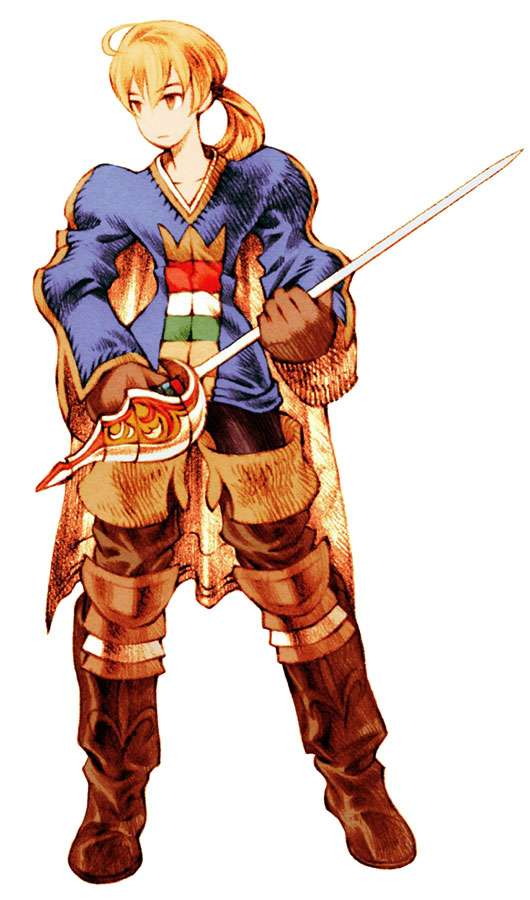
\includegraphics[width=0.85\columnwidth]{./art/worldbook/ramza.jpg}\end{center}
%
%
\accf{A cisão de Glabados (1167 A.C. -- 1250 A.C.)}\\
Em 1171, a igreja de Glabados executou \accf{Orran Durai} como um traidor após escrever os Escritos de Durai.
Isto causou agitação entre os vários padres ordenados e um deles, Karling Nox, iniciou um movimento em Limberry, o qual clamava por reforma dentro da igreja, procurando, em suas palavras, um "retorno ao verdadeiro caminho de Sto.~Ajora".
Isso se espalhou por Ordalia e várias províncias orientais de Ivalice, após a igreja ter declarado o estado de Nox como de um herético, o padre começou a juntar uma quantidade de seguidores considerável.
Sentindo a oportunidade de tomar terras e riquezas da igreja, vários barões e condes declararam sua conversão a esta nova interpretação da fé de Ajora e deram abrigo aos novos convertidos.
Enfraquecido pelos eventos da Guerra do leão, Glabados estava incapaz de evitar a ascenção dos alto proclamandos Ajoranos e esta divisão religiosa se manteve crescendo pelos próximos 80 anos. Em contraste, o governo da dinastia Heiral se provou ser infeliz em manter o poder centralizado e teve que fazer várias concessões à nobreza a fim de manter sua posição como rei de Ivalice.
Estas concessões aumentaram a decentralização do reino, empoderando lordes locais.
Em 1240, as tensões religiosas se tornaram violentas, com as hostilidades entre os seguidores de Glabados e de Ajora, levando a várias escaramuças de pequena escala, culminando no massacre de Yardrow em 1243, onde uma multidão matou uma congregação de 500 fiéis Ajoranos durante um ritual religioso.
Isto gerou vários tratados de defesa mútuos entre os novres, criando ambos a \accf{Liga Glabados}, liderada pelo grande duque Rudolph Barrington de Fovoham e a \accf{Liga Ajorana}, liderada pelo marquÊs Henry Elmdore de Limberry.
A criação dessas duas ligas somente aumentou a tensão posteriormente, mas pelos próximos sete anos a paz reinou em Ivalice.
Em 1250, se seguida a uma doença severa, o rei Luther Heiral ficou em um estado de coma.
Seu sobrinho, Paul Heiral, que era um devoto fervoroso da fé de Glabados, foi designado como o regente.
Temendo ser perseguido por suas crenças religiosas, a Liga Ajorana votou por uma guerra de precaução contra o regente, com a intenção de o trocar por outro nobre que fosse mais simpático com a fé ajorana.
Em resposta, a Liga Glabados reuniu suas tropas e isto afundou Ivalice numa guerra civil.
%
\vfill
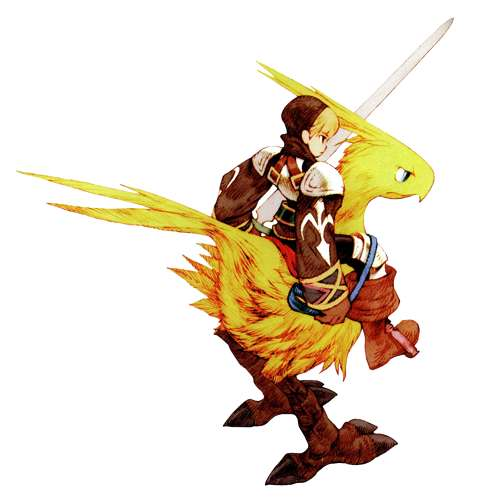
\includegraphics[width=\columnwidth]{./art/worldbook/chocoborider.jpg}
%
\clearpage
%
\ofsubsubsection{Cronologia}
%
\newcommand{\tltitle}[1]{\mbox{\accf{#1}}}
\newcommand{\nlwb}{\vfill}
%
\tltitle{< 2000 B.C.} Os primeiros assentamentos dos caçadores coletores se forma. A metalurgia e a magia são descobertas.\nlwb
%
\tltitle{\textasciitilde 700 B.C.:} O império Ronan, qu reinou do palácio de Ronan, é varrido por uma doença misteriosa. \nlwb
%
\tltitle{\textasciitilde 600 B.C.:} O império Ronan se separa em 4 países: o reino de Barron, o reino de Palmecia e o de Melmond. A tecnologia e militarismo se desenvolvem rapidamente. \nlwb
%
\tltitle{\textasciitilde 500 B.C.:} Lucavi assola o mundo. 
Um grande herói e seus doze companheiros derrotam o Lucavi, eles se ficam conhecidos como os Bravos zodíacos.
O Sacro império de Ydoran surge das cinzas do destruído reino de Barron. 
\nlwb
%
\tltitle{\textasciitilde 200 B.C.:} O Sacro império de Ydoran conquista o império de Palmecia e Melmond. O monastério de Orbonne é construído. \nlwb
%
\tltitle{50 B.C.:} O Santo Ajora naxe em Bervenia. \nlwb
%
\tltitle{22 B.C.:} O Santo Ajora é enviado como um espião do Sacro império de Ydoran, prega sobre o Paraíso, em segredo junta as pedras do zodíaco e junta seus 13 discípulos.\nlwb
%
\tltitle{1 B.C.:} O Santo Ajora é enforcado no cadafalso d Golgollada pelo Sacro império de Ydoran. Um desastre afunda partes de Mullonde, formando o mar de coral negro. \nlwb
%
\tltitle{0 B.C.:} O Cataclismo acontece. Moogles, pessoas aladas e outras civilizações são varridas. O herói rei, Mesa Rixksen, salva a humanidade. O Sacro império de Ydoran é destruído.\nlwb
%
\tltitle{25 A.C.:} Os discípulos restantes do Sto. Ajora formam a igreja de Glabados, que se estabelece como o maior poderio de Ivalice por muitos séculos.\nlwb
%
\tltitle{150 A.C.:} A Cidade de Yardrow é estabelecido.\nlwb
%
\tltitle{\textasciitilde 300 A.C.:} A igreja de Glabados extende sua influência através das facções separatistas. Eles expulsão o clero de Phara de Ivalice, os quais acabam ajudando a criar Ordalia.\nlwb
%
\tltitle{610 A.C.:} A casa Atkascha unifica os sete reinos em guerra, estabelecendo o reino de Ivalice.\nlwb
%
\tltitle{1014 A.C.:} O reino de Ordalia anexa o estado independente de Zelmonia. \nlwb
%
\tltitle{1108 A.C.:} Druksmald Goltanna, filho do duque Goltanna e primo de Ondoria III, nasce, assim como Cidolfus Orlandeau, filho do conde Orlandeau.\nlwb
%
\tltitle{1113 A.C.:} Goffard Gaffgarion nasce. O rei Devanne III de Ordalia, morre sem um sucessor. O rei Denamda Atkascha II de Ivalice, proclama a si mesmo como herdeiro e declara guerra. A guerra dos cinquenta anos se inicia. \nlwb
%
\tltitle{1113 A.C:} Ivalice conquista Zelmonia. O rei Denamda II morre em Viura, capital de Ordallia. Denamda Atkascha III é coroado rei de Ivalice. Batalhas entre Ivalice e Ordallia continuam enquanto o rei Varoi VI de Ordallia tenta afastar as forças Ivalicianas de Zelmonia. \nlwb
%
\tltitle{1127 A.C.:} Bestrald Larg, filho do duque Larg e parente do Ondoria Atkascha III, nasce. Dycedarg Beoulve, primogênito do lorde Barbaneth Beoulve, nasce.\nlwb
%
\tltitle{1129 A.C.:} Messam Elmdore, filho do marquês Elmdore, nasce, Gustav Margriff e Ondoria Atkascha III, filhos de Denamda Atkascha IV, nascem.
%
\newpage
%
\tltitle{1133 - 1136 A.C.:} Bestrald Larg se alia a Dycedarg Beoulve. Wiegraf Folles e Zalbaag Beoulve, filhos do lorde Beoulve, nascem. \nlwb
%
\tltitle{1137 A.C.:} Ordallia força as forças Ivalicianas de volta a Zelmonia. Décadas de batalhas se seguem entre eles. Louveria Larg, filha do duque Larg, nasce. \nlwb
%
\tltitle{1139 A.C.:} As forças Romandas invadem Ivalice através do estreito de Rhana. A fortaleza de Ziekden é constrúida. Orran Durai nasce.\nlwb
%
\tltitle{1142 -- 1144 A.C.:} Ivalice recupera o controle do castelo de Riovanner dos invasores Romandos, que recuam de Ivalice. O conde Cidolfus Orlandeau se alia ao duque Druksmald Goltanna. Agrias Oaks nasce.\nlwb
%
\tltitle{1147 A.C.:} O duque Bestrald Larg se torna o general da Ordel de cavaleiros do céu nortenho. Delita Heiral nasce.\nlwb
%
\tltitle{1149 A.C.:} Ovelia Atkascha, filha do rei Denamda IV, Alma Beoulve, quarta criança de Barbaneth Beoulve e Tietra Heiral nascem. \nlwb
%
\tltitle{1155 -- 1157 A.C.:} Zalbaag Beoulve se torna comandante da Ordem do céu nortenho. Ele acolhe sob sua custódia Delita e Tietra. O rei Denamda Atkascha IV de Ivalice morre. Ondoria III é coroado rei da casa Atkascha. O príncipe LEnnar de Ordallia invade Zelmonia e Zeltennia. O rei Ondoria III se casa com Louveria Larg e ele se torna a rainha.\nlwb
%
\tltitle{1162 A.C.:} Ovelia Atkascha é adotada pelo rei Ondoria III. O pai de Orran Durai é morto à serviço do conde Orlandeau, o conde o adota. \nlwb
%
\tltitle{1163 A.C.:} O príncipe Orinus Atkascha, filho do rei Ondoria III, nasce. Ramza Beoulve e Delita Heiral entram na Academia militar de Gariland. O Lorde Barbanth Beoulve é envenenado. Goddard Gaffgarion é expulso da Ordel do céu oriental. 
Veteranos dos Homens mortos são dispensados sem pagamento, eles protestam e formam a Brigada cadáver. \nlwb
%
\tltitle{1164 -- 1166 A.C.:} A guerra dos leões se inicia sobre o sucessor do rei Ondoria III entre os cavaleiros do céu nortenho, do duque Larg e a Ordem de cavaleiros do céu austral, do duque Goltanna. 
Ambos são mortos pelos traidores Dycedarg e Delita, respectivamente. A rainha Louveria é aprisionada.
Ramza Beoulve impede um massacre no Forte Basselat e para a ressurreição de Ultima pelo Lucavi.
\nlwb
%
\tltitle{1166 A.C.:} Delita Heiral se casa com Ovelia Atkascha e é coroado rei de Ivalice. A igreja de Glabados se aproveita da situação para recuperar seu poder.
\nlwb
%
\tltitle{1171 A.C.:} Orran Durai escreve os Escritos de Durai e é executado como um traidor pela igreja de Glabados.\nlwb
%
\tltitle{1173 A.C.:} Karling Nox escreve pela reforma da igreja e é declarado como um herético. Muitos nobres de Ordalia e de Ivalice oriental se convertem à nova fé Ajorana.\nlwb
%
\tltitle{1243 A.C.:} 500 fiéis Ajoranos são massacrados em Yardrow. A liga Ajorana e a liga de Glabados são fundadas.
As tensões aumentam de início, mas a paz se estabelece por um tempo.
\nlwb
%
\tltitle{1250 A.C.:} Paul Heiral sucede seu pai como o regente. Temendo perseguição, a liga Ajorana declara guerra, começando com a Guerra da cisão.
%
\clearpage
%
%
\ofsubsubsection{Geografia}
%
\ofimagewide{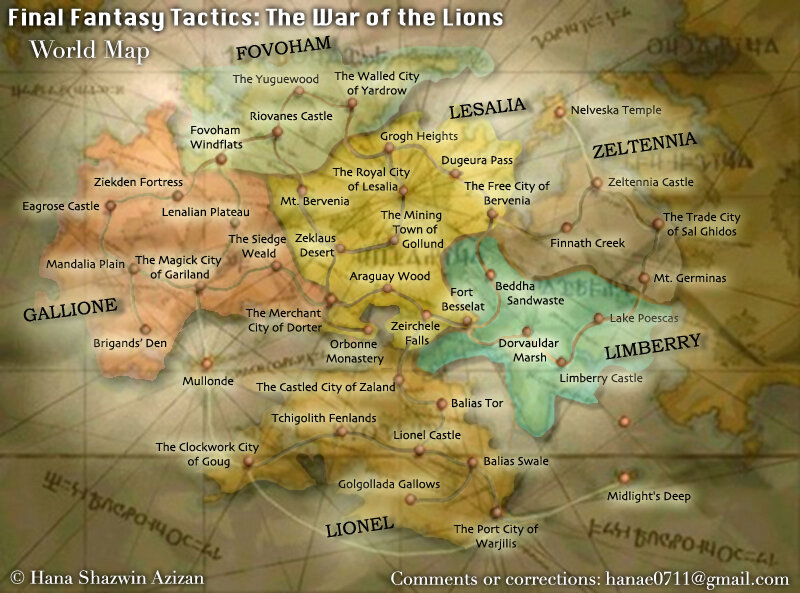
\includegraphics[width=\textwidth]{./art/worldbook/map.jpg}} 	
%
\vspace*{\fill}
%
\accf{\large Fovoham} é um território mais na parte mais ao norte de Ivalice. Governado pelo grande duque Rudolph Barrington, é separado da nação militar de Romanda pelo estreito de Rhana.
Fovoham desempenhou um importante papel em deter a invasão Romanda na Guerra dos cinquenta anos, graças ao grande duque e seus esquadrão de assassinos, os Khamja. Atualmente, é a principal força por trás da liga de Glabados, e alguns até mesmo dizem que o regente real, Paul Heiral, nada mais é do que uma marionete do grande duque. 
\accf{Castelo Riovanes} é o lar e fortaleza do grande duque Barrington. 
Este castelo se distingue por suas torres ao estilo Romando.
Sua posição permite não somente uma ótima posição defensiva, mas também o controle de todas a rotas comerciais através do norte de Ivalice, como a Montanha~Bervenia serve de barreira natural para a movimentação de mercadorias e tropas.
\accf{A Cidade murada de Yardrow}, também conhecida como a Cidade fortaleza de Yardrow, é localizada ao leste do castelo Riovannes e ao norte da Cidade real de Lesalia. É uma cidade fortificada com alguns séculos de história, protegida por espessas muralhas de pedra para repelir invasores.
Esta cidade é tem um passado importante por ter protegido as partes mais setentrionais de Fovoham e ao ter imposto uma considerável ameaça aos ataques vindo do estreito de Rhana.
Por séculos, a família real confiou a essa cidade somente o seus vassalos mais leais, por ser também o principal local para um ataque surpresa contra a capital.
%
\newpage
%
\vspace*{\fill}
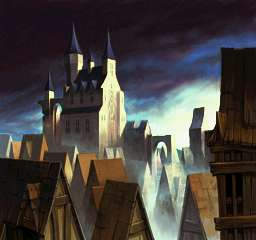
\includegraphics[width=\columnwidth]{./art/worldbook/riovanes.jpg}
%
\vfill
\ofquote{"Nossa nação existe somente por causa do povo! Existimos por causa deles."}{Cidolfus Orlandu}
%
\clearpage
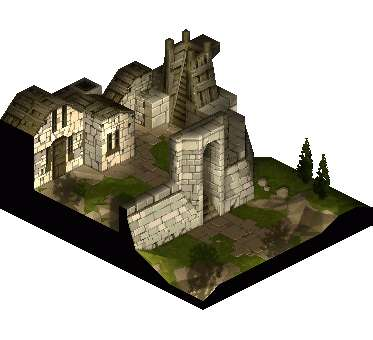
\includegraphics[width=\columnwidth]{./art/worldbook/yardrow.jpg}
\vfill
%
\accf{A floresta Yugue}, também conhecido como a floresta Yuguo, é localizada ao leste do castelo Riovannes. 
As árvores de dois séculos de idade ainda crescem aqui, mas mesmo sua floresta antiga não foi poupada pela fúria da guerra.
Embora, a floresta possa ser uma ótima fonte de materiais de construção, rumores de fantasmas que assombram suas árvores mantém qualquer um de as usar, exceto pelos mais corajosos ou estúpidos lenhadores.
\accf{As planícies ventania de Fovoham}, também conhecida como as planícies de Fovoham, localizada ao leste da fortaleza de Ziekeden e é o local dos moinhos ventania, também conhecidos como cabanas do moinho.
Estas vastas planícies são cobertas por grama baixa e açoitada por fortes ventos vindos do estreito de Rhana.
Eles são a principal área de cultivo do grande ducado, provendo alimento não somente para o castelo Riovannes, mas também para o castelo Igros.
%
\vfill
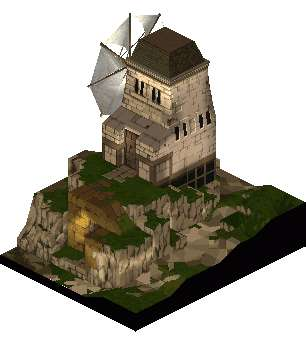
\includegraphics[width=\columnwidth]{./art/worldbook/fovohamplains.jpg}
\newpage
%
\accf{\large Gallionne} é um ducado no reino de Ivalice.
Governado pelo duque Lestrad Larg e é localizado em Ivlaice ocidental.
Suas fronteiras são o mar ao oeste e ao sul, Fovoham ao nordeste e Lesalia ao leste. Seu centro de poder é no castelo Eagrose.
Assim sendo, foi mantida pela Ordem de cavaleiros do céu nortenho durante a Guerra dos leões.
Lestrad é um bastião aliado do grande duque Barrington e apoia a liga de Glabados na guerra que se seguirá.
%
\vfill
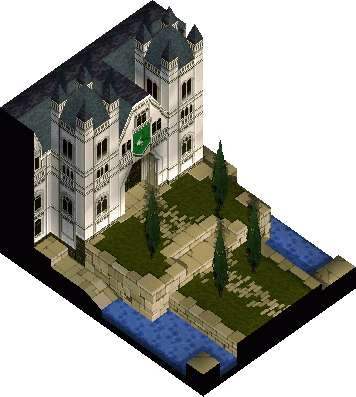
\includegraphics[width=\columnwidth]{./art/worldbook/belouveresidence.jpg}
\vfill
%
\accf{Castelo Eagrose}, também conhecido como castelo Igros, é a sede de Gallione e lar do duque Larg, seu lorde.
Esta cidade é a segunda em tamanho, somente perdendo para a Cidade real de Lesalia.
Durante a Guerra do leão, foi a base da casa Beoulve e da Ordem do cé sententrional.
Também é o local onde o demônio Lucavi, Adrammelech, foi derrotado.
\accf{A Cidade mágika de Gariland}, também conhecida como a Cidade mágica de Gariland, é o lar da Academia real para as artes magikas, famosa por produzir Elidibus, um herói mago da Guerra dos cinquenta anos.
Localizada à leste do castelo Eagrose e a oeste da cidade mercantil de Dorter.
Durante a Guerra do leão, foi controlado pela Ordem do céu nortenho e contém a academia onde Ramza Veoulve e Delita Heiral foram treinados.
\accf{A Cidade mercantil de Dorter}, também conhecida como a cidade do mercantil de Dorter, é uma cidade que se desenvolveu como o núcleo para o comércio terrestre.
É um local cheio de vida, frequentado por todo tipo de comerciante.
Localizado ao leste da Cidade magika de Gariland e ao norte do monastério de Orbonne, é a maior encruzilhada de Ivalice.
Também é o lar da maior congregação dos fiéis Ajoranos em Gallione assim como o maior oponente à influência de Glabados.
%
\newpage
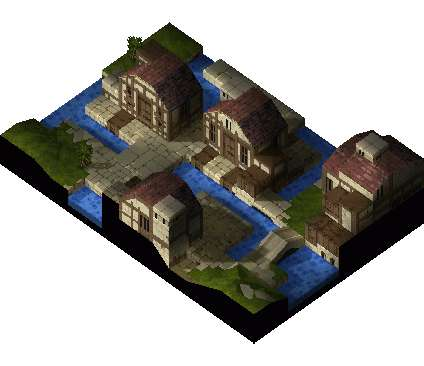
\includegraphics[width=\columnwidth]{./art/worldbook/gariland.jpg}
\vfill
%
\accf{Fortaleza de Ziekden}, também conhecida como o forte Zeakden, é uma fortaleza construída durante a Guerra dos cinquenta anos a fim de evitar a invasão Romanda através do estreito de Rhana. Fica localizada ao leste do castelo Eagrose.
Atualmente, esta em grande parte indefesa, pois há poucas hostilidades entre Romanda e Ivalice, mas caso caia a qualquer inimigo de Gallione ou Fovoham, pode se tornar uma fortificação importante.
\accf{O covil dos bandidos}, também conhecido como o forte dos ladrões, é uma pequena estrutura construída sobre um cais, logo ao sul do castelo Eagrose.
Já fora um refúgio para pescadores, e foi, por um tempo, o lar de bandidos: o caos que seguiu a Guerra dos cinquenta anos o tornou em um notável esconderijo de ladrões, além de ser utilizado pela Brigada cadáver como sua fortaleza.
Após a Guerra dos leões ter terminado, ela foi novamente ocupada por pescadores e é parte de uma importante rota para Mullonde.
\accf{Planícies Mandalia} é um local famosa por seus grandes pináculos de calcário que emergem do solo como presas de uma grande besta.
%
\vfill
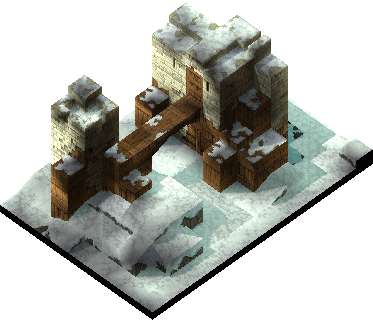
\includegraphics[width=\columnwidth]{./art/worldbook/zeakden.jpg}
\newpage
%
Seu calcário branco parece presas, o que lhe dá o nome de "planícies da besta". Está localizada ao sudeste do castelo Eagrose e a oeste da Cidade mercantil de Dorter.
\accf{A mata Siedge}, também conhecida como Bosque Sweegy, é uma floresta antiga rodeada por montanhas.
Rumores contam que ela já foi habitada por Moogles.
Está localizada a leste da Cidade Magika de Gariland e a oeste da Cidade mercantil de Dorter.
\accf{Platô Lenaliano}, também conhecida como o Platô de Lenalia, é um platô árido pontilhado com rochas dentadas, mas com pouca flora.
Está localizada ao norte da Cidade Magika de Gariland e ao sul das planícies ventania de Fovoham.
Como ela conecta o coração do território de Gallione com Fovoham, é uma importante rota comercial que conecta Dorter ao norte de Ivalice.
%
\ofpar
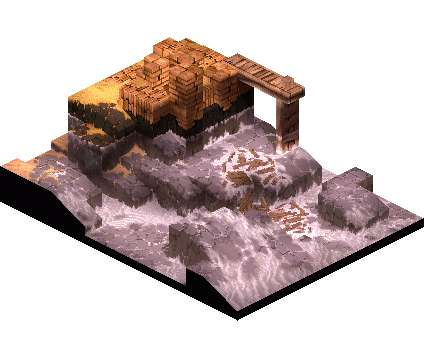
\includegraphics[width=\columnwidth]{./art/worldbook/poeskas.jpg}
\ofpar
%
\accf{\large Limberry} é a região mais oriental de Ivalice, governada pelo marquês Henry Elmdore, o jovem neto de Messam Elmdore, um dos heróis da Guerra dos cinquenta anos, que defendeu as fronteiras de Ivalice contra os invasores Romandos.
\accf{Castelo Limberry} é uma fortificação da família Elmdore, um belo castelo alvo que jaz às margens do Lago Dolla.
Henry Elmdore, que experienciou menos do que vinte invernos, governa essa terra com a paixão e fervor religioso que somente os jovens podem juntar.
Seu pai convidou o próprio Nox para ser seu conselheiro em sua corte e foi o primeiro governante a abraçar a reforma Ajorana.
Desde da conversão de seu pai, sua recém fortuna têm ajudado a tornar Limberry em um poderio econômico e as terras que costumavam ser controladas pela igreja estão mais produtivas do que nunca.
\accf{Brejo Dorvauldar}, também conhecido como o Pântano Dolbodar, é uma rica terra pantanosa a leste de Limberry.
O rio Dorvauldar carrega o solo fértil daque até as planícies.
Está localizada entre o Forte Besselat e o castelo de Limberry.
Nos últimos 60 anos, houveram intensos esforços de construção, originando represas e canais de irrigação, domando-se a maior parte das velhas áreas de pântano e criando uma importante área arável, transformando-o no celeiro de Limberry.
\accf{Lago Poescas} já fora um grande corpo d'água, mas agora não passa de um leito de lago coberto de sal branco.
Está localizado logo ao leste do castelo de Limberru e é assombrado pelos mortos vivos.
Assim como a maioria das fronteiras entre Zeltennia e Limberry, é um terreno baldio desprovido de muita importância econômica e política.
O sal é minerado de suas bordas, mas o medo dos mortos vivos impede que esta área se torne a principal produtora deste produto.
%
\vfill
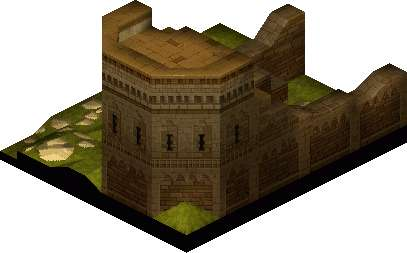
\includegraphics[width=\columnwidth]{./art/worldbook/bethla.jpg}
\vfill
%
\accf{O deserto de areia de Beddha}, também conhecido como o deserto selvagem que cobre a maior parte ocidental de Limberry, localizado ao norte do forte Besselat da Ordem do céu austral, e das tumbas dos imperadores antigos podem ser vistas soterradas na areia.
Antes do Cataclismo, ele costumava ser um importante local do Sacro império, mas foi transformada de terras agrícolas exuberantes em um deserto arenoso quase que da noite para o dia.
Caravanas viajam através dele constantemente, por ser parte de uma importante rota comercial que conecta o nordeste de Ivalice e Lionel.
\accf{Forte Besselat}, também conhecido como a guarnição Bethla, foi uma fortificação da Ordem do céu austral.
Está localizado entre o brejo de Dorvadar e as cataratas de Zeirchele.
Ele jaz dentro das terras reais de Lesalia, mas foi tomado num ataque surpresa das forças Ajoranas e está sob a ocupação de Limberry.
A ocupação de Bethla marca o início da Guerra da cisão e sua posição estratégica vigia a maioria da rotas comerciais terrestres que passam por Lionel.
%
\vfill
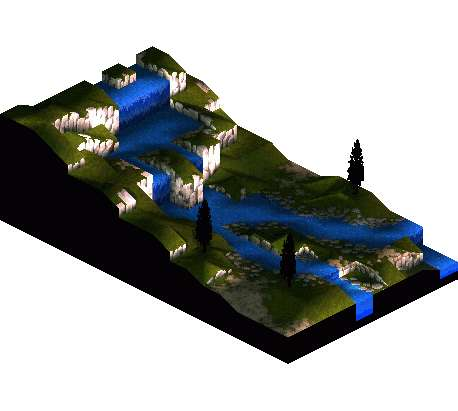
\includegraphics[width=\columnwidth]{./art/worldbook/finath.jpg}
\newpage
%
\accf{\large Zeltennia} é um ducado localizado no leste de Ivalice, junto ao vizinho Limberry. Zeltennia é governada pelo velho Jotan Goltanna, o filho caçula de Druksmald Goltanna, que lutou na Guerra dos cinquenta anos, um descendente do último rei Denamda II.
Situada na fronteira mais oriental de Ivalice, Zeltennia foi conhecida como o campo de batalha mais terrível durante a Guerra dos cinquenta anos.
Está propensa a invasão pelo reino de Ordallia e foi quase que totalmente perdida para este, não fosse pelas defesas lideradas pelo Cidolfus Orlandeau, um cavaleiro a serviço da casa Goltanna.
Atualmente, está ao lado de Limberry na liga Ajorana.
\accf{Castelo Zeltennia} é uma fotificação da casa Goltanna. Foi altamente reforçada durante a Guerra dos cinquenta anos e agora é uma fortaleza formidável.
A conversão do Goltanna à fé Ajorana não nasceu da fé, mas da conveniência, pois o governador de Zeltennia se viu cercado por crentes Ajoranos tanto pelo sul quanto pelo leste, ele previu o potencial de ganhos ao se juntar à liga e a guerra se assomava no horizonte.
\accf{Cidade comercial de Sal Sal Ghidos}, também conhecida como a Cidade comercial de Zarghidas, é o ponto de partida do comércio entre Zeltennia e Ordallia.
Após os eventos da Guerra dos cinquenta anos, caiu em decadência, pois as relações azedas entre Ivalice e Ordallia bloquearam a maior parte do comércio. Contudo, em seguida à cisão e com a recém descoberta riqueza nas áreas pantanosas de Dorvaudar, ela vivenciou a renascença e atualmente se enche de atividade. 
%
\ofpar
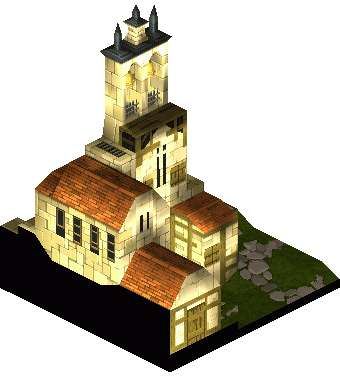
\includegraphics[width=\columnwidth]{./art/worldbook/zeltenniachapel.jpg}
\ofpar
%
\accf{O riacho Finath}, também conhecido como o rio Finath, está localizado entre a Cidade livre de Bervenia e o castelo de Zeltennia.
É um recurso defensivo importante, bloqueando o avanço dos exércitos que poderiam enviar um ataque da Cidade livre de Bervenia.
Sabendo disso, Goltanna posicionou a maioria de seus exércitos na posição defensiva nos bancos de areia, incerto de se ele deveria atravessar a terra imperial - uma hesitação que não passou despercebida por seus aliados.
\accf{Monte Germinas}, também conhecido como os Picos Germinas, está na parte mais ao leste de Ivalice. Marca o ponto mais alto da cadeia de montanhas que pontilham a fronteira oriental de tanto Zeltennia quanto Limberry, direcionando a maioria do comércio para as proximidades da Cidade de sal Ghidos.
Seus picos congelados são a fonte da maioria dos rios que já preencheram o lago Pescas, mas agora rumam ao oeste até o rio Finath.
%
\ofpar
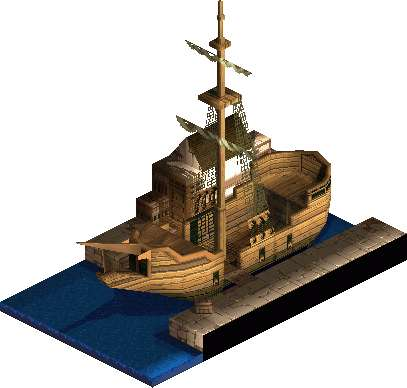
\includegraphics[width=\columnwidth]{./art/worldbook/warjilis.jpg}
\ofpar
%
\accf{\large Lionel} é um dos sete territórios de Ivalice. já fora conhecida como a terra do Sacro império de Ydoran e o centro dos ensinamentos antigos, conhecidos como Pharismo.
Ambos sucumbiram após a catástrofe que se abateu sobre a capital, a qual ocorreu logo após a execução do Sto. Ajora Glabados, que é uma figura central das fés de Glabados e Ajorana.
Antes da Guerra do leão, Lionel continuou seu papel como um território religioso, governado pelo cardeal Delacroix, uma figura proeminente na igreja e um dos heróis da Guerra dos cinquenta anos.
Depois da guerra, com o colapso do poderio de Glabados, Lionel foi reformada em um ducado secular, fornecido à família Lenande pelos reis Heiral.
É também o local da captura do Santo Ajora Glabados e da batalha de Ramza Beoulve contra Cúchulainn.
Lionel é atualmente neutra na Guerra da cisão e emissários de ambas as ligas Glabados e Ajorana tentaram o seu melhor a fim de persuadir o duque a se juntar à luta.
\accf{A Cidade fortificada de Zaland} também conhecida como a Cidade forte de Zaland, é uma cidade elevada, construída no topo de uma baixa montanha e serve de portão de entrada à província de Lionel.
Está localizada na única terra que conecta lionel ao continente de Ivalice e sua importância estratégica para todo o ducado é primordial.
\accf{A Cidade portuária de Warjilis}, também conhecida como a Cidade mercantil de Warjilis, está localizada ao sul do castelo Lionel ao longo da costa.
Como a única Cidade mercantil em Lionel, esta cidade desenvolveu um ponto de transito para comércio no Mar de Bugross.
Warjilis é um porto importante não somente para Lionel, amas também para todo o reino de Ivalice e a frota de Lionel estacionada lá é de longe a frota naval mais poderosa de toda a região.
\accf{A Cidade mecânica de Goug}, também conhecida como a Cidade máquina de Goug, é uma cidade mineradora localizada na parte mais ao sul de Lionel.
Ela produz armas mecânicas com a tecnologia de velha geração. Diz-se que as ruínas de uma civilização perdida jaz enterrada abaixo das ruas de Goug, relíquias da era do Santo Ajora, quanto aeronaves incontáveis preenchiam os céus e os homens de ferro caminhavam pelas ruas das cidades.
Mas é uma arte da fabricação de tais coisas se perdeu, se sequer existiram.
\accf{Os patíbulos Golgollada}, também conhecido como o Local de execução de Golgorand, é o local de execução do Sto. Ajora Glabados.
Está localizado ao sul do castelo de Lionel e é usado como um lugar de execução pública pela província.
\accf{Alagados Tchigolith}, também conhecido como Pântano Zigolis, está localizado ao oeste do castelo de Lionel e ao leste da Cidade mecânica de Goug.
Incontáveis pessoas morream aqui durante a Guerra dos cinquenta anos, mudando sua planície já fértil em um alagado venenoso.
Mesmo agora, mais de um século depois da guerra, as cicatrizes não sanaram e rumores de que alguma magia profana foi liberada lá circula entre o povo.
%
\vfill
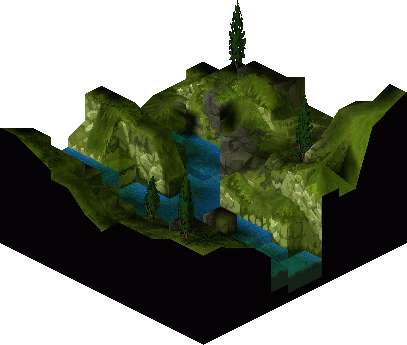
\includegraphics[width=\columnwidth]{./art/worldbook/bariaus.jpg}
\vfill
%
\accf{Balias Tor}, também conhecida como as Colinas Bariaus, está localizada ao norte do castelo Lionel. Foi aqui que o Sacro império de Ydoran condenou Balias, o primeiro dos discípulos do Santo Ajora, à morte.
É um local sagrado para ambas as fés de Glabados e Ajorana.
\accf{Valas Balias}, também conhecida como o Vale Bariaus, está localizado  entre o castelo Lionel e o a Cidade portuária de Warjilis. É o vale árido onde Balias, o primeiro dos discípulos do Santo Ajora, se escondeu de seus perseguidores do Sacro império de Ydoran.
\accf{Catedral Mullonde}, também conhecida como o Tempo do Sto.~Murond, é o principal centro da igreja de Glabados e jaz numa ilha a oeste do continente de Lionel.
Uma vez já um arcebispado independente, Mullonde foi incorporada ao ducado de Lionel após a Guerra do leão, mas permanece sob o controle da igreja.
%
%
\clearpage
%
\accf{\large Lesalia} é o centro do reino de Ivalice em Final Fantasy Tactics. Foi a sede da família real de Atkscha, que governou desta região mesmo durante a Guerra dos cinquenta anos e a Guerra dos leões, mas agora abriga a família real Heiral.
Os sinais de riqueza e luxo persistiram mesmo quando Ivalice ter enfrentado guerra após guerra.
\accf{A Cidade real de Lesalia}, também conhecida como a Capital imperial de Lesalia, é a capital do reino de Ivalice.
É a principal sede da coroa e suas protegem o luxuoso forte que abriga a família real de Ivalice.
Pelo rei estar em coma e Paul heiral, o regente, dançar conforma a música tocada pelo grande duque de Fovoham, as terras reais estão alinhadas com a liga de Glabados, mas a inabilidade do regente para coordenar seus exércitos tem levado a muitas vitórias Ajoranas recentes.
Se ele puder juntar forças com os principais exércitos de Glabados, a maré dessa guerra pode mudar.
\accf{A Cidade mineradora de Gollund}, também conhecida como a Goland, a cidade do carvão, está localizada ao sul da Cidade real de Lesalia e contém uma grande mina de carvão.
Rica em recursos minerais, estas planícies onde a cidade jaz também é maltratada por tempestades de neve que duram o ano todo.
\accf{A Cidade livre de Bervenia}, famosa por ser a terra natal do Santo Ajora Glabados, está sob o controle direto da igreja de Glabados.
Está localizada na estrada entre a Cidade real de Lesalia e o Castelo Zeltennia.
É o caminho mais direto de Zeltennia à capital, mas não foi atacada até agora.
%
\ofpar
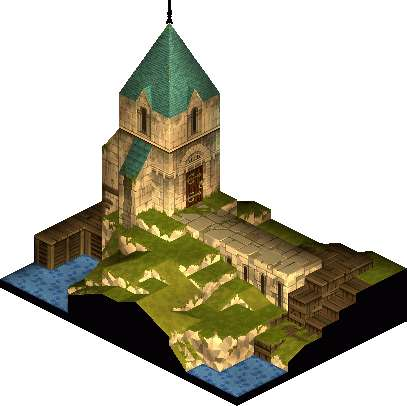
\includegraphics[width=\columnwidth]{./art/worldbook/orbonne.jpg}
\ofpar
%
\accf{Monastério Orbonne} foi construída há mais de doze século atrás e está sob o controle da igreja de Glabados.
Contém o Armazém de livros subterrâneo, uma misteriosa biblioteca que possui velhos tomos da era do Sto.~Ajora.
Diz-se que está preenchida com muitas obras literárias, tais quais os escritos históricos e manuscritos, incluindo obras em línguas estrangeiras.
As obras literárias estão espalhadas em pilhas bagunçadas pelo chão e pergaminhos antigos e litografias estão pilhadas entre obras impressas.
Os padres são impedidos de ir ao terceiro andar subterrâneo.
Na área mais profunda do cofre, os andares cobrem um túnel de entrada e um runa mágica está escrita no piso.
\accf{O deserto Zeklaus} jaz ao norte da Cidade mercantil de Dorter, na estrada para a Cidade real de Lesalia, e é a localização do Sietch do rato d'areia, onde o marquês Elmdore foi mantido como refém pela Brigada cadáver.
Escaldante durante o dia e congelante à noite, não é mistério do porquê tão poucos viajam por esse deserto. Por causa disso, a maioria do comércio que vei de Lesalia usa Fovoham como rota ao invés de passar pela rota mais direta por Dorter.
%
\vfill
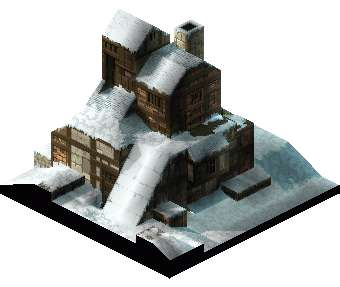
\includegraphics[width=\columnwidth]{./art/worldbook/goland.jpg}
\vfill
%
\accf{Monte Bervenia}, também conhecido como o Vulcão Bervenia, é o maior vulcão em atividade em Ivalice e está localizado a sudeste do Castelo Riovannes. Lava derretida flui descendo pela sua superfície, cinzas brancas e fumaça escurecem o céu.
É a segunda razão pela qual Zeklaus não é usada como uma rota comercia, exceto por contrabandistas e os mercadores mais audazes.
\accf{Florestas Araguay} está localizado ao leste da Cidade mercantil de Dorter e é uma extensa floresta que cobre a região mais ao sul de Lesalia. Habitada por uma grande variedade de faunas raras.
Sua madeira é famosa em toda Ivalice e muito delas adornam os mais ricos castelos do reino.
\accf{Montes Grogh}, também conhecido como as Colinas Grog, está localizado entre a Cidade real de Lesalia e a Cidade murada de Yardrow.
Os montes compõem o maior cinturão de terras agrícolas da região de Lesalia e a maioria das plantações colhidas aqui são destinadas à capital.
É uma das mais velas e mais desenvolvidas regiões agrícolas de todo o reino.
\accf{Cataratas Zeirchele}, também conhecida como as Quedas Zirekile, é uma grande cachoeira localizada a oeste do Forte Besselat. Poucos podem evitar se encantar pela vista de suas cascatas que descem as escadas como das montanhas Algost.
As águas caem em direção ao leste até Limbery para alimentar os ricos de Dorvaudar.
\accf{Passagem Dugeura}, também conhecida como Passo Dogoula, está localizada na estrada entre o Castelo Riovanies e o Castelo Zeltennia.
Aproximadamente 2.000 dohms de altura, o Monte Landria já foi usado pelos monges como um local sagrado de jejum e expiação.
Esta passagem é a rota mais segura entre a região de Grog e Bervenia e mesmo uma pequena força poderia defendê-la de um ataque, caso necessário.
%
%
\clearpage
%
\ofsubsubsection{Ideias de camapanhas}
%
\onecolumn
%
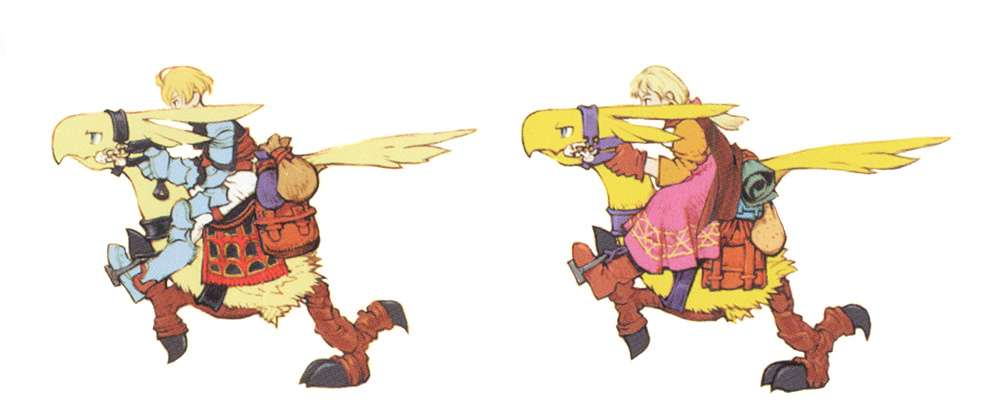
\includegraphics[width=\textwidth]{./art/worldbook/chocobos.jpg}
%
\vfill
%
\begin{multicols}{2}
%
\accf{Ideia de campanha - Herós mitológicos:}
Situada na Era dos mitos, os jogadores explorarão os contos dos lendários heróis de Barron, Paramecia, Kushuka e Melmond. Esta era se parece com as histórias tradicionais a Final Fantasy, por incluir temas de armas, magia e alta fantasia.
Ganchos de aventura incluoem as guerras entre os reinos, a descoberta das ruínas Ronan e artefatos, a revolução Kushuka e a luta dos primeiros Bravos zodíacos contra Lucavi e seus demônios.
%
\ofpar
%
\accf{Ideia de campanha - A intriga de Ydoran:}
O Sacro império de Ydoran foi um lugar muito atribulado. Havia nobres e intrigas da corte em abundância, e enquanto tinha o mais alto nível de tecnologia e magia da era anterior, a ordem social estrita e o punho de ferro impostas por seus governantes em sua rápida conquista, fez deste lugar um candidato prioritário para espionagem e dramas sociais.
Junto a isso, as cinco décadas antes do Cataclismo também presenciaram a ascensão do Sto. Ajora, que também era um espião Ydorano.
Muitos conflitos religiosos com o debate de Pharism contra Ajora, assim como a segunda conspiração de Lucavi, fez deste um cenário para aventuras.
%
\ofpar
%
\accf{Ideia de campanha - O Cataclismo:}
Se inicia com a execução do Sto. Ajora, esta campana explora os eventos a cerca do tempo do Cataclismo.
Portanto, a estória pode dar uma ideia do tamanho e da súbita destruição de uma das mais avançadas civilizações da história de Ivalice.
Os jogadores serão heróis que lutarão juntamente ao herói rei Mesa para salvar a humanidade e, possivelmente, também as outras raças de Ivalice dos efeitos do Cataclismo.
Nesta aventura ao sobrenatural, eles terão de enfrentar campeões divinos e catástrofes e, talvez, até mesmo os próprios deuses.\\
%
\columnbreak\\
%
\accf{Ideia de campanha - Reinos em guerra:}
Situada entre os primeiro e o quinto séculos depois do Cataclismo, este gancho de campanha explora os conflitos entre os seis reinos de Kaladis e a ascensão à proeminência de Mullonde e da Igreja de Glabados.
Neste momento do tempo, Lesalia, Fovoham, Zeltennia, Gallione, Lionel e Limberry eram reinos independentes, forjando alianças e guerreando constantemente entre si.
Diferente das eras anteriores, não havia mais não humanos e a alta magia, com o nível de tecnologia regredindo ao ponto comparável aos períodos iniciais da era medieval.
%
\ofpar
%
\accf{Ideia de campanha - Guerras de Ivalice:}
Esta ideia de campanha se situa nos sessenta anos entre as duas maiores guerras de Ivalice já sofridas: a Guerra dos cinquenta anos e a Guerra dos leões.
Este período pode ser visitado tanto para recriar os eventos do jogo eletrônico de outro ponto de vista, quanto para explorar contos não cantadas de heróis de ambos os lados do conflito.
Como a vida dentro de Romanda e o resultado de sua derrota?
Quais vozes dentro da Igreja imploravam por razão antes de começarem a conspirar a Guerra do leão?
Como que o povo reagiu após à queda da Brigada cadáver?
Estas questões podem garantir que estórias interessantes sejam contadas.
%
\ofpar
%
\accf{Ideia de campanha - A cisão:}
Este é o cenário padrão para esta enciclopédia, situado em 1250 A.C.
A cisão entre as fés Ajorana e de Glabados acendem as tensões fundamentais do reino, levando à formação de duas ligas religiosas.
A qual lado os jogadores se aliarão neste conflito?
Como as outras nações irão responder à fraqueza de Ivalice?
Quais são os motivos secretos da maioria dos participantes políticos?
%
\end{multicols}
%
\vfill
%
\hspace*{\fill}\ofquote{"Uma pedrinha pode somente fazer uma ondulação a princípio, mas gerar uma onda algum dia."}{Wiegraf Folles}\hspace*{\fill}\\
%
\twocolumn
\clearpage
%
%\ofsubsubsection{Optional Rules}
%%
%The following is a collection of optional rules and content, which you can use to create a closer feeling to Final Fantasy Tactics.
%%
%\vfill
%%
%\accf{Grid-based Combat:}
%You can use a square grid to visualize combat in the same manner as FFT.
%Each square is 1u by 1u in size and player characters take up 1 square of space.
%The distance between two squares is the sum of the horizontal and vertical squares between them, this system is called the \accf{Manhattan~distance}.
%In other words, adjacent squares to your up, down left and right have a distance of 1u from you, but adjacent diagonal ones have a distance of 2u.
%Ranges and target distances for abilities are adjusted accordingly.
%The example below shows the normal (2u) target shape, as well as the special shapes line (5u) and front (2u). 
%The blue squares represent the caster, while the red ones represent enemy combatants.
%%
%\vfill
%%
%\begin{figure}[h!]
%	\centering
%	\begin{tikzpicture}[]
%	\tikzstyle{filled}=[draw, black!50!white, rectangle, thin, minimum height = 0.5cm, minimum width=0.5cm]
%	\tikzstyle{target}=[fill=red!20!white]
%	\tikzstyle{caster}=[fill=blue!60!white]
%	\tikzstyle{enemy}=[fill=red!80!white]	
%	\draw[step=0.5,black!50!white, thin,xshift=-0.25cm,yshift=-0.25cm] (0,0) grid (9, 3.5);	
%	%Normal
%	\node[filled, caster](g0)at (1, 0) {};
%	\node[filled, enemy](g0)at (1, 2) {};
%	\node[filled, enemy](g0)at (0, 1) {};
%	\node[filled, target](g0)at (1, 1) {};
%	\node[filled, target](g0)at (1, 1.5) {};
%	\node[filled, target](g0)at (1, 2.5) {};
%	\node[filled, target](g0)at (1, 3) {};
%	\node[filled, target](g0)at (1.5, 2.5) {};
%	\node[filled, target](g0)at (0.5, 2.5) {};
%	\node[filled, target](g0)at (1.5, 1.5) {};
%	\node[filled, target](g0)at (0.5, 1.5) {};
%	\node[filled, target](g0)at (1.5, 2) {};
%	\node[filled, target](g0)at (2, 2) {};
%	\node[filled, target](g0)at (0, 2) {};
%	\node[filled, target](g0)at (0.5, 2) {};
%	%Line
%	\node[filled, caster](g0)at (4, 0) {};
%	\node[filled, enemy](g0)at (4, 1.5) {};
%	\node[filled, enemy](g0)at (4.5, 2.5) {};
%	\node[filled, target](g0)at (4, 0.5) {};
%	\node[filled, target](g0)at (4, 1) {};
%	\node[filled, target](g0)at (4, 2) {};
%	\node[filled, target](g0)at (4, 2.5) {};	
%	%Front
%	\node[filled, caster](g0)at (7.5, 0) {};
%	\node[filled, enemy](g0)at (8, 1) {};
%	\node[filled, enemy](g0)at (6.5, 1.5) {};	
%	\node[filled, target](g0)at (7.5, 0.5) {};
%	\node[filled, target](g0)at (7.5, 1) {};
%	\node[filled, target](g0)at (7.5, 1.5) {};
%	\node[filled, target](g0)at (8, 0.5) {};
%	\node[filled, target](g0)at (8.5, 0.5) {};
%	\node[filled, target](g0)at (7, 0.5) {};
%	\node[filled, target](g0)at (6.5, 0.5) {};
%	\node[filled, target](g0)at (7, 1) {};
%	\end{tikzpicture}
%\end{figure}
%%
%\vfill
%%
%\accf{Directional Defense:}
%In conjunction with a square grid, you can also change the potency of a combatant's defense depending on the direction they are attacked from.
%At the end of every turn, combatants have to announce the direction that they are facing. 
%There are 4 possible directions (up, down, left and right), so the one they are facing is their front, the opposite direction is their back and the two remaining directions are their sides. 
%Whenever combatants are Attacked from a side, their DEF is halved when calculating the suffered damage.
%Whenever combatants are Attacked from behind, their Evasion DC is increased by 2 while trying to evade the Attack.
%%
%\vfill
%%
%\accf{Monsters of Ivalice:}
%Below are examples of monsters that are common in the world of Ivalice.
%Apart from these, the following monsters from the bestiary supplement may also be encountered:
%Skeleton, Ghoul, Cockatrice, Ahriman, Coeurl, Mindflayer, Malboro, Behemoth, Red Dragon.
%%
%\vfill
%%
%\ofmonster{Floating Eye}{4}{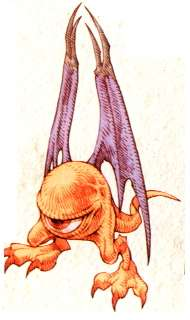
\includegraphics[width=0.16\columnwidth]{./art/worldbook/eye.jpg}}
%{
%	HP: & \hfill 32 & MP: & \hfill 30 \\
%	STR: & \hfill 2 & DEF: & \hfill 2 \\
%	MAG: & \hfill 5 & RES: & \hfill 4 \\
%	AGI: & \hfill 4 & Size: & \hfill S\\
%}
%{\accf{Beam}: 2d DMG, 3u Range \hfill \accf{Immune:}\sleep\silence\blind}
%{	
%	\mtech{Wing Buffet}{5}{0r}{3u (front)}{Self}{Enemies in the target area suffer 2d wind damage.}{}
%}
%%
%\newpage
%%
%\ofmonster{Goblin}{2}{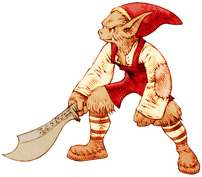
\includegraphics[width=0.26\columnwidth]{./art/worldbook/goblin.jpg}}
%{
%	HP: & \hfill 16 & MP: & \hfill 18\\
%	STR: & \hfill 2 & DEF: & \hfill 1 \\
%	MAG: & \hfill 0 & RES: & \hfill 0 \\
%	AGI: & \hfill 3 & Size: & \hfill M\\
%}
%{\accf{Knife}: 1d DMG \hfill \accf{Immune:}\poison\immobile}
%{
%	\mtech{Goblin Punch}{2}{0r}{Single}{Weapon}{Make an Attack against the target. If you hit, you push him back by 1u on top of the damage dealt.}{}		
%	\mtech{Spin Punch}{4}{0r}{1u}{Self}{Make an Attack against everyone within 1u.}{}		
%}
%%
%\vfill
%%
%\ofmonster{Red Chocobo}{3}{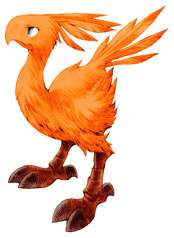
\includegraphics[width=0.18\columnwidth]{./art/worldbook/chocobo-red.jpg}}
%{
%	HP: & \hfill 28 & MP: & \hfill 16\\
%	STR: & \hfill 3 & DEF: & \hfill 2 \\
%	MAG: & \hfill 1 & RES: & \hfill 1 \\
%	AGI: & \hfill 4 & Size: & \hfill M\\
%}
%{\accf{Beak}: 1d DMG \hfill \accf{Resilient}:\fire}
%{	
%	\mtech{Choco Kick}{4}{0r}{Single}{Weapon}{The target suffers 3d damage and is knocked back by 1u.}{}
%	\mreaction{Choco Counter}{Whenever you are hit by an Attack, immediately makean Attack on the perpetrator.}
%}
%%
%\vfill
%%
%\ofmonster{Grenade}{4}{
\includegraphics[width=0.22\columnwidth]{./art/worldbook/bomb.jpg}}
%{
%	HP: & \hfill 35 & MP: & \hfill 20\\
%	STR: & \hfill 2 & DEF: & \hfill 2 \\
%	MAG: & \hfill 0 & RES: & \hfill 1 \\
%	AGI: & \hfill 3 & Size: & \hfill M\\
%}
%{
%	\accf{Tackle}: 2d DMG \hfill \accf{Resilient}:\fire \hfill \accf{Weak}:\ice\water
%}
%{
%	\mtech{Flame Attack}{5}{0r}{Single}{2u}{The target suffers 3d fire damage.}{\fire}		
%	\mtech{Self-Destruct}{0}{1r}{2u}{Self}{Inflict KO on yourself to deal 6d fire damage to everyone within the target area.}{\fire}		
%}
%%
%\vfill
%%
%\ofmonster{Revenant}{5}{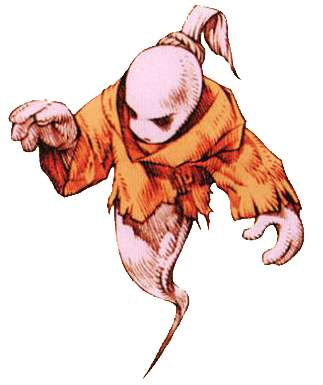
\includegraphics[width=0.2\columnwidth]{./art/worldbook/ghost.jpg}}
%{
%	HP: & \hfill 50 & MP: & \hfill 40\\
%	STR: & \hfill 3 & DEF: & \hfill 3 \\
%	MAG: & \hfill 5 & RES: & \hfill 6 \\
%	AGI: & \hfill 2 & Size: & \hfill M\\
%}
%{
%	\accf{Touch}: 2d DMG \hfill \accf{Weak}:\holy \hfill \accf{Immune:}\poison\immobile\sleep
%}
%{
%	\mtech{Zombie Touch}{4}{0r}{Single}{Weapon}{Make an Attack against the target. If you hit, he suffers Zombie for 10 rounds on top of the damage dealt.}{}	
%	\mtech{Drain Touch}{5}{0r}{Single}{Weapon}{Make an Attack against the target. If you hit, increase your HP by 1d on top of the damage dealt.}{}	
%}
%%
%\clearpage
%%
%\accf{Bravery \& Faith:} 
%To create more heroic moments in your adventure, you can allow characters to derive special powers from their Bravery or Faith.
%Every character tracks one resource pool for each, that can hold up to 5 points.
%Players roll 1d for each during character creation to determine their starting Bravery and Faith (a 6 is rounded down to a 5).
%Characters recover 1 point of Bravery and 1 point of Faith whenever they go to sleep and they can never spend more than 1 point of either at once.
%\accf{Bravery} allows characters to channel their inner courage to reach beyond their usual abilities.
%Characters can spend 1 point of Bravery whenever they perform a check to add 1 to the result of their roll.
%They can also spend 1 point of Bravery whenever they deal any damage during combat to add 1d to the total damage dealt.
%When a character's Bravery drops to 0, all of their total damage dealt is halved.
%The GM can award additional points of Bravery whenever someone acts particularly heroic or deduct a point when they act cowardly.
%\accf{Faith} helps characters to overcome failures through confidence in their beliefs.
%Characters can spend 1 point of Faith whenever they perform a check to re-roll one die after seeing the result.
%They can also spend 1 point of Faith whenever they suffer any damage during combat to reduce the total damage suffered by 1d.
%The GM can award additional points of Faith whenever someone acts in accordance to their belief system and deduct a point when they act against it.
%When a character's Faith drops to 0, they have Disadvantage on every check that they perform.
%%
%\vfill
%%
%\ofquote{"Most people have to act the roles given to them. Then again, most of them haven't even noticed they're acting."}{Delita Hyral}
%%
%\vfill
%%
%\accf{Hiring Soldiers:} 
%In the world of Ivalice, many capable combatants will offer their services for the right price.
%As such, the party can hire paid soldiers in almost any major city to improve their combat strength.
%These soldiers are controlled by the GM during battles and generally should not play a major role outside of it.
%Accordingly, you also do not need to track their current experience and progression. 
%For characters of greater importance, we recommend to use the standard character creation rules, if necessary you
%can convert a hired soldier to a fully fledged character later on.
%When using the \accf{Bravery \& Faith} rules, a hired soldier will immediately leave the party when either their Bravery or Faith drops to 0.
%On the right are some examples of soldiers that can be hired, along with their required daily salary.
%As these are very common types of combatants, you can also use them as human enemies.
%%
%%
%%
%\newpage
%%
%\ofmonster{Squire}{1}{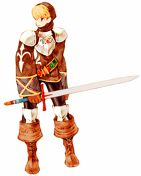
\includegraphics[width=0.22\columnwidth]{./art/worldbook/squire-male.jpg}}
%{
%	HP: & \hfill 15 & MP: & \hfill 12\\
%	STR: & \hfill 2 & DEF: & \hfill 1 \\
%	MAG: & \hfill 0 & RES: & \hfill 0 \\
%	AGI: & \hfill 3 & Size: & \hfill M\\
%}
%{\accf{Sword}: 1d DMG \hfill \accf{Salary:} 25G per day}
%{
%	\mtech{Throw Stone}{2}{0r}{Single}{3u}{The target suffers 1d damage.}{}
%	\ofrow\accf{Items:} 1x Potion		
%}
%%
%\vfill
%%
%\ofmonster{Chemist}{2}{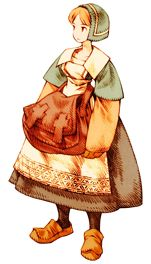
\includegraphics[width=0.14\columnwidth]{./art/worldbook/chemist-female.jpg}}
%{
%	HP: & \hfill 2 & MP: & \hfill 26\\
%	STR: & \hfill 1 & DEF: & \hfill 1 \\
%	MAG: & \hfill 1 & RES: & \hfill 1 \\
%	AGI: & \hfill 2 & Size: & \hfill M\\
%}
%{\accf{Knife}: 1d DMG \hfill \accf{Salary:} 50G per day}
%{
%	\mtech{Aid}{4}{0r}{Single}{1u}{Remove one negative Status Effect from the target except KO.}{}	
%	\mreaction{Auto-Potion}{Whenever an ally within 1u suffers damage, you can immediately use an Item on them.}		
%	\ofrow\accf{Items:} 3x Potion, 1x Phoenix Down, 1x Remedy
%}
%%
%\vfill
%%
%\ofmonster{Archer}{3}{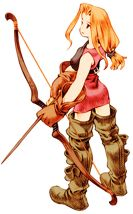
\includegraphics[width=0.16\columnwidth]{./art/worldbook/archer-female.jpg}}
%{
%	HP: & \hfill 27 & MP: & \hfill 18\\
%	STR: & \hfill 1 & DEF: & \hfill 1 \\
%	MAG: & \hfill 0 & RES: & \hfill 1 \\
%	AGI: & \hfill 2 & Size: & \hfill M\\
%}
%{\accf{Bow}: 2d DMG, 5u range \hfill \accf{Salary:} 100G per day}
%{
%	\mtech{Aim}{2}{0r}{Single}{Self}{On the next Attack that you perform, the target has Disadvantage on the evasion check.}{}	
%	\ofrow\accf{Items:} 2x Potion, 1x Eyedrops	
%}
%%
%\vfill
%%
%\ofmonster{Knight}{4}{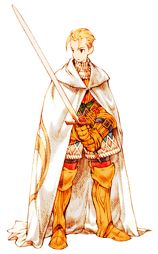
\includegraphics[width=0.17\columnwidth]{./art/worldbook/knight-male.jpg}}
%{
%	HP: & \hfill 38 & MP: & \hfill 25\\
%	STR: & \hfill 4 & DEF: & \hfill 2 \\
%	MAG: & \hfill 0 & RES: & \hfill 1 \\
%	AGI: & \hfill 3 & Size: & \hfill M\\
%}
%{\accf{Sword}: 2d DMG \hfill \accf{Salary:} 150G per day}
%{
%	\mtech{Rend Power}{5}{0r}{Single}{Weapon}{
%		Make an Attack against the target.  If you hit, the damage dealt is halved and the target suffers DeSTR for 3 rounds.
%	}{}	
%	\mtech{Rend Magick}{5}{0r}{Single}{Weapon}{
%		Make an Attack against the target.  If you hit, the damage dealt is halved and the target suffers DeMAG for 3 rounds.
%	}{}	
%	\ofrow\accf{Items:} 1x Hi-Potion, 1x Remedy	
%}
%%
%\clearpage